\documentclass[12pt, twoside]{article}
\usepackage[letterpaper, margin=1in, headsep=0.5in]{geometry}
\usepackage[english]{babel}
\usepackage[utf8]{inputenc}
\usepackage{amsmath}
\usepackage{amsfonts}
\usepackage{amssymb}
\usepackage{tikz}
%\usetikzlibrary{quotes, angles}

\usepackage{graphicx}
\usepackage{enumitem}
\usepackage{multicol}

\usepackage{fancyhdr}
\pagestyle{fancy}
\fancyhf{}
\renewcommand{\headrulewidth}{0pt} % disable the underline of the header

\fancyhead[LE]{\thepage}
\fancyhead[RO]{\thepage \\ Name: \hspace{4cm} \,\\}
\fancyhead[LO]{BECA / Dr. Huson / Geometry\\* Unit 6: Distance \& slope\\* 15 January 2019}

\begin{document}
\subsubsection*{7.10 Do Now: Transformations}
  \begin{enumerate}

  \item Apply a dilation mapping $\triangle ABC \rightarrow \triangle A'B'C'$ with a factor of $k=2$ centered at $(3,3)$. Draw and label the image on the grid and make a table of the coordinates.
    \begin{flushright} %4 quadrant regents grid w T-Chart
    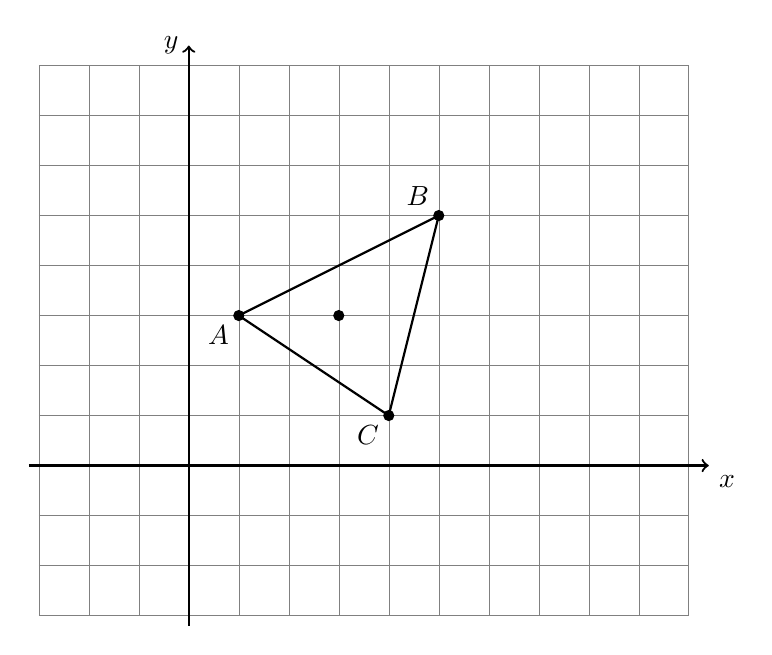
\begin{tikzpicture}[scale=.635]
      \draw [help lines] (-3,-3) grid (10,8);
      \draw [thick, ->] (-3.2,0) -- (10.4,0) node [below right] {$x$};
      \draw [thick, ->] (0,-3.2)--(0,8.4) node [left] {$y$};
      \draw [thick] (1,3)--(4,1)--(5,5)--cycle;
      \draw [fill] (1,3) circle [radius=0.1]node[below left]{$A$};
      \draw [fill] (4,1) circle [radius=0.1]node[below left]{$C$};
      \draw [fill] (5,5) circle [radius=0.1]node[above left]{$B$};
      \draw [fill] (3,3) circle [radius=0.1];
    \end{tikzpicture}
    \end{flushright}
    
  \item Find the image of $P(3,5)$ after a reflection over the $x$-axis.  \vspace{2cm}

  \item What transformation maps $\triangle ABC$ onto $\triangle DEF$, shown below? Fully specify the transformation.
    \begin{flushright}
      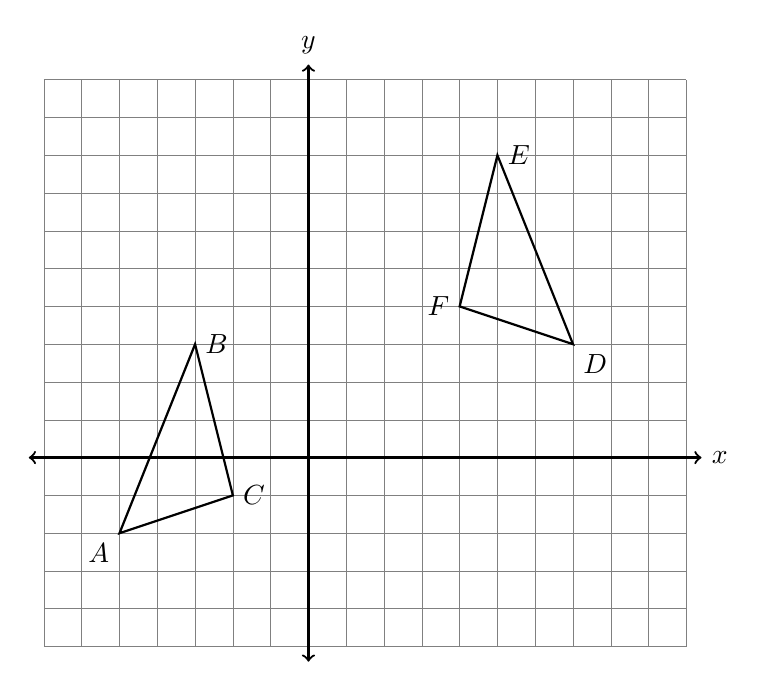
\begin{tikzpicture}[scale=.48]
      \draw [help lines] (-7,-5) grid (10,10);
      \draw [thick, <->] (-7.4,0) -- (10.4,0) node [right] {$x$};
      \draw [thick, <->] (0,-5.4)--(0,10.4) node [above] {$y$};  
      \draw [thick]
      (-5,-2) node[below left] {$A$}--
      (-3,3) node[right] {$B$}--
      (-2,-1) node[right] {$C$}--cycle;  
      \draw [thick]
      (7,3) node[below right] {$D$}--
      (5,8) node[right] {$E$}--
      (4,4) node[left] {$F$}--cycle; 
    \end{tikzpicture}
  \end{flushright}

\newpage
  \item Plot two transformations. Rotate $\triangle ABC$ clockwise $90^\circ$ around the origin, then reflect the result across the $x$-axis. Make a table of the coordinates and plot and label the images on the axes. %$\triangle ABC \rightarrow \triangle A'B'C'$ 
  \begin{flushright}
    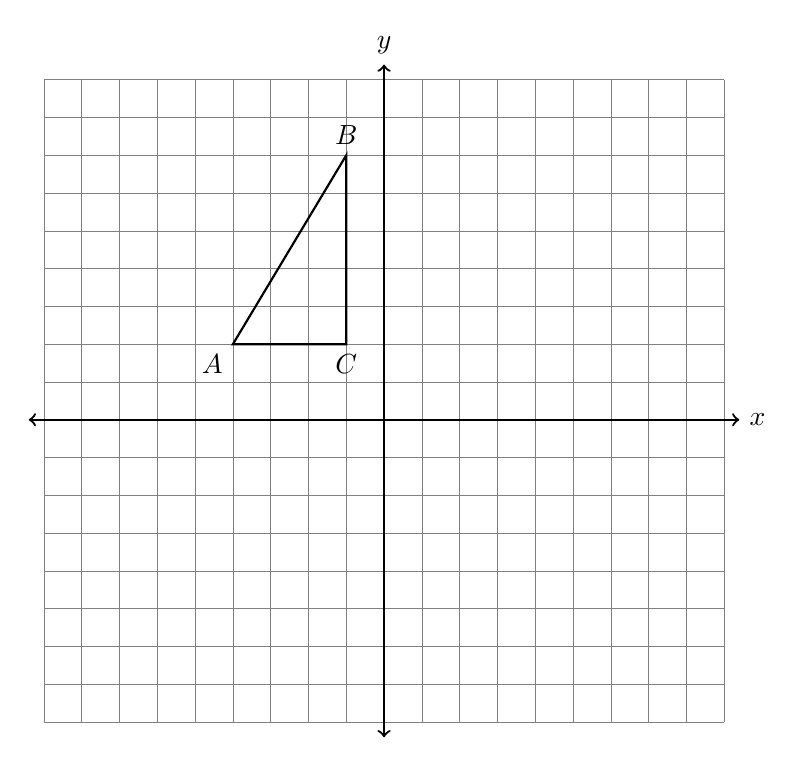
\begin{tikzpicture}[scale=.48]
      \draw [help lines] (-9,-8) grid (9,9);
      \draw [thick, <->] (-9.4,0) -- (9.4,0) node [right] {$x$};
      \draw [thick, <->] (0,-8.4)--(0,9.4) node [above] {$y$};  
      \draw [thick]
        (-4,2) node[below left] {$A$}--
        (-1,7) node[above] {$B$}--
        (-1,2) node[below] {$C$}--cycle;  
  \end{tikzpicture}
  \end{flushright}

  \item A translation maps $A(-2, 1) \rightarrow A'(5,1)$. What is the image of $B(3,-1)$ under the same translation? \vspace{1cm}

  \item Reflect $\triangle ABC$ over the $y$-axis. Plot and label the image on the axes and make a table of the coordinates showing $\triangle ABC \rightarrow \triangle A'B'C'$.
  \begin{flushright}
      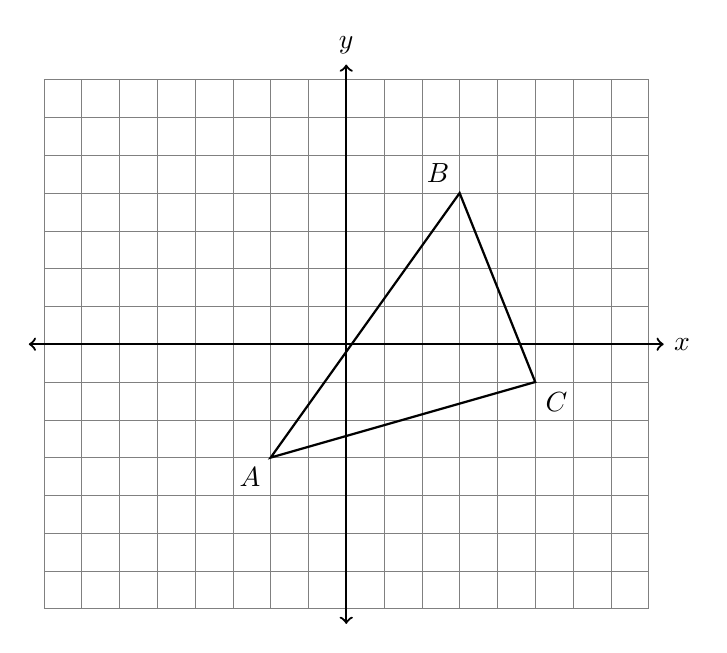
\begin{tikzpicture}[scale=.48]
      \draw [help lines] (-8,-7) grid (8,7);
      \draw [thick, <->] (-8.4,0) -- (8.4,0) node [right] {$x$};
      \draw [thick, <->] (0,-7.4)--(0,7.4) node [above] {$y$};  
      \draw [thick]
        (-2,-3) node[below left] {$A$}--
        (3,4) node[above left] {$B$}--
        (5,-1) node[below right] {$C$}--cycle;  
    \end{tikzpicture}
  \end{flushright}

\end{enumerate}
\end{document}